% Failure taxonomy of holdout 3: Gap clusters, Gap rows by evidence in context, and partial-answer causes.
% Bars: 0.2 cm per row. Label column 5.6 cm wide.
\begin{figure}[htbp]
\centering
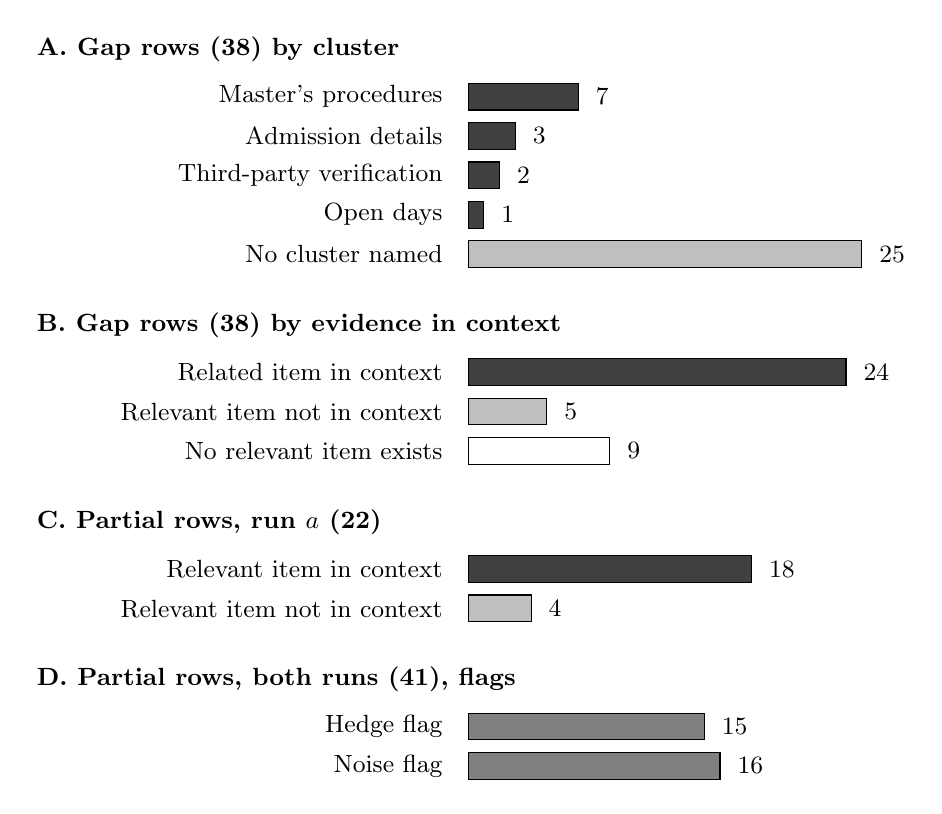
\begin{tikzpicture}[x=1cm,y=1cm,font=\small]
  % panel A
  \node[anchor=west] at (-5.6,0) {\textbf{A. \textsc{Gap} rows (38) by cluster}};
  \foreach \y/\lab/\n/\sty in {
      -0.6/{Master's procedures}/7/black!75,
      -1.1/{Admission details}/3/black!75,
      -1.6/{Third-party verification}/2/black!75,
      -2.1/{Open days}/1/black!75,
      -2.6/{No cluster named}/25/black!25} {
    \node[left] at (-0.2,\y) {\lab};
    \fill[\sty,draw=black] (0,\y-0.17) rectangle ({0.2*\n},\y+0.17);
    \node[right] at ({0.2*\n+0.1},\y) {\n};
  }
  % panel B
  \node[anchor=west] at (-5.6,-3.5) {\textbf{B. \textsc{Gap} rows (38) by evidence in context}};
  \foreach \y/\lab/\n/\sty in {
      -4.1/{Related item in context}/24/black!75,
      -4.6/{Relevant item not in context}/5/black!25,
      -5.1/{No relevant item exists}/9/white} {
    \node[left] at (-0.2,\y) {\lab};
    \fill[\sty,draw=black] (0,\y-0.17) rectangle ({0.2*\n},\y+0.17);
    \node[right] at ({0.2*\n+0.1},\y) {\n};
  }
  % panel C
  \node[anchor=west] at (-5.6,-6.0) {\textbf{C. \textsc{Partial} rows, run $a$ (22)}};
  \foreach \y/\lab/\n/\sty in {
      -6.6/{Relevant item in context}/18/black!75,
      -7.1/{Relevant item not in context}/4/black!25} {
    \node[left] at (-0.2,\y) {\lab};
    \fill[\sty,draw=black] (0,\y-0.17) rectangle ({0.2*\n},\y+0.17);
    \node[right] at ({0.2*\n+0.1},\y) {\n};
  }
  % panel D
  \node[anchor=west] at (-5.6,-8.0) {\textbf{D. \textsc{Partial} rows, both runs (41), flags}};
  \foreach \y/\lab/\n/\sty in {
      -8.6/{Hedge flag}/15/black!50,
      -9.1/{Noise flag}/16/black!50} {
    \node[left] at (-0.2,\y) {\lab};
    \fill[\sty,draw=black] (0,\y-0.17) rectangle ({0.2*\n},\y+0.17);
    \node[right] at ({0.2*\n+0.1},\y) {\n};
  }
\end{tikzpicture}
\caption[Where answers were lost on holdout 3, as row counts]{Where answers were lost on holdout 3, as row counts. Panel A: the \textsc{Gap} rows (38 in each run) that belong to the four clusters that added data could fill. The other 25 rows are not assigned to a cluster. Panel B: the same \textsc{Gap} rows of run $a$ by whether a relevant item was in the agent's context. The relevant items are mostly related passages that lack the specific fact. Panel C: the \textsc{Partial} rows of run $a$ by evidence in context. Panel D: the hedge flags (vague wording that avoids stating a rule) and noise flags (unneeded or off-topic detail) among the 41 partial answers of the two runs combined, with each flag counted separately. Relevance comes from AI judges (Section~\ref{sec:live-recall}).}
\label{fig:failure-taxonomy}
\end{figure}
